\documentclass{mpaper}

\begin{document}

\title{Data-flow compilation of Fortran for FPGAs}
\author{James Macdonald}
\matricnum{2126890}

\maketitle

\begin{abstract}
According to Simon Peyton Jones, an abstract should address
four key questions. First, what is the problem that this
paper tackles? Second, why is this an interesting problem?
Third, what is the solution this paper proposes?
Finally, why is the proposed solution a good one?
\end{abstract}

\section{Introduction}

Computer simulation has long been a corner stone of cutting edge scientific and engineering work. Simulators allow scientists and engineers to test their theories and designs far more rapidly than the physical world allows. One of the most striking examples of advanced simulation in our everyday lives is the forecasting of extreme weather events. The need for better predictions of environmental events such as hurricanes has always been apparent. The death and destruction brought by these events means any increase in accuracy forecasting the epicentre of the storm and lengthening the warning time that can be given to residents can save a huge number of lives. As extreme weather events become more frequent and severe due to climate change, the need for high-resolution forecasts is at an all time high.

Simulation systems also usually comprise of preforming the same series of operations on many points, over many time steps. This makes them ideal candidates for optimisation. Many of the computer models used for simulation tasks are legacy systems, often written in languages such as Fortran. Though these models maybe classed as legacy in terms of software engineering they are battle tested and are known to provide accurate results. Furthermore, many new models are being developed by scientists who still use Fortran. As a language, Fortran provides a number of primitives that are useful for scientific code, while also being familiar to scientists who have other priorities other than learning new languages and cutting edge computer science techniques.


FPGAs provide an exciting, new avenue in the world of high-performance computing (HPC). Results show they can offer huge performance increases, while also drastically reducing energy consumption. FPGAs have long been a feature of hardware development work flows and working with them required expert knowledge of hardware description languages such as Verilog or VHDL. Recently, efforts have been made to open up access to FPGAs by integrating them with the OpenCL parallel programming framework. Although this lowers the bar to entry significantly it still requires expertise and careful structuring of programs in order to take full advantage of execution on a FPGA.

When these factors are considered together it becomes clear that novel ways of marrying up the power of FPGAs with the wealth of Fortran simulation codes would be extremely beneficial. If a turn-key solution for porting these simulators to FPGAs was available, scientists would be able to run faster, higher-accuracy simulations, while reducing energy usage with next to no additional effort on their part.

This paper presents a \textit{refactoring compiler} than analyses scientific simulation code written in Fortran and outputs refactored Fortran that is suitable for high performance execution using FPGA devices. The process outlined in this paper requires no changes to be made to the input source.

%%%%%%%%%%%%%%%%%%%%%%%%%%%%%%%%%%%%%%%%%%%%%%%%%%%%%%%%%%%%%%%%%%%
\subsection{Problem Statement}

This project aiomsd

\subsection{Aims}

This project aims to create a compiler capable of compiling Fortran scientific simulation codes to OpenCL optimised for execution on FPGA devices.

The output from this compiler will be a Fortran OpenCL dialect that can be converted to standard OpenCL C using an existing compiler \cite{VanderbauwhedeDavidson2018}. The output from this existing compiler can then be used as input to the FPGA vendor's HLS flow \cite{IntelCorporation, Xilinx}. The HLS flow will then produce a bitstream that can be executed by the FPGA.

If successful this project will significantly reduce the burden in porting legacy Fortran simulators such as the 2D Shallow Water Model \cite{Hall2009} and the Large Eddy Simulator for Urban Flows \cite{Nakayama2011} for acceleration using FPGAs. This could potentially unlock huge increases in performance with minimal manual effort.


%%%%%%%%%%%%%%%%%%%%%%%%%%%%%%%%%%%%%%%%%%%%%%%%%%%%%%%%%%%%%%%%%%%
\section{Background Survey}

\subsection{Fortran Refactoring}

Fortran has always been highly popular with the scientific community and continues to be so today  \cite{VanderbauwhedeDavidson2018}. As such, there have been many attempts to create automated refactorings to improve execution performance and aid maintainability.

One of the first papers to suggest refactoring Fortran to increase performance was by Overby et al (2005) \cite{Overbey2005}. When refactoring to improve performance the paper suggests defining a set of just-in-time refactorings to be applied just before compilation. This is recommended because many of the refactorings necessary to improve performance adversely affect the readability of the code. The researchers present an Eclipse-based Fortran IDE called Photran that can perform these refactorings. While the authors of Photran suggest a framework for applying performance focused refactorings to Fortran code, they do not actually specify what refactorings will be available. They make reference to unrolling loops as an example but do not provide any concrete examples of how they would apply this to take advantage of new accelerator types such as GPUs or FPGAs. This is obviously a major limitation when it comes to accelerating real world systems as any user of the IDE would have to write the acceleration refactorings themselves. This limits the value of the IDE because producing these refactorings will likely be as much work as rewriting the simulator using a parallel processing framework such as OpenCL.

Other work in this area has been carried out by researchers at Cambridge university. They released a paper in 2013 detailing their work on CamFort \cite{Orchard2013}. In this work they describe a Haskell DSL they have created for refactoring Fortran. The researchers demonstrate their work by introducing automated refactorings such as removing equivalence statements and common blocks as these are features that can lead to data aliasing and are often a source of subtle bugs. The authors report that the Haskell DSL is an effective way to express refactorings, however the scope of the refactorings they have implemented is limited. In the future work section, CamFort's authors suggest that, using the DSL, refactorings could be created that allow loops to be parallelised and run on GPUs. However, creating refactorings to enable GPU offload is likely to be significantly more work than just refactoring to code that is destined to be compiled and executed on the original target device.

In their paper ``Semi-automatic porting of a large-scale Fortran CFD code to GPUs'' \cite{Corrigan2012} the authors propose a system to allow the FEFLO CFD simulator \cite{Lbhner2001} to be ported for execution on GPUs via CUDA and the Thrust library \cite{Library}. The compiler is developed in Python, and is specifically designed to only work with the FEFLO codebase. OpenMP \cite{OpenMP} annotations already present in the FEFLO code are used by the compiler to produce CUDA kernels. The authors make it clear they have not developed a general purpose auto-parallelizing compiler. They state the main goal of the work is to allow the FEFLO developers to continue developing in Fortran, while allowing users of the simulator to take advantage of modern GPU hardware. One limitation, that they acknowledge, is that their approach is focused only on porting the FEFLO simulator. As the compiler is only designed to work with one codebase the authors discuss heuristics that are used as part of its operation. Reliance on FEFLO specific heuristics means it is likely to be difficult to extend the compiler to work with other projects in the future. One final issue with the work is that it relies heavily on the Thrust library which requires CUDA, and therefore only NVIDIA GPUs are supported. This significantly limits the range of GPUs that the ported code can be used with.

In their paper ``Domain-specific acceleration and auto-parallelization of legacy scientific code in Fortran 77 using source-to-source compilation''\cite{VanderbauwhedeDavidson2018} the authors present a three-phase compile, that takes Fortran 77 code as input and outputs OpenCL code optimised for execution using a GPU. The first phase of the multi-stage compile is performed by a refactoring compiler which runs to clean up and convert Fortran 77 input code to Fortran 95. It finds and removes some potentially problematic coding practices allowed in Fortran 77. For example, the compiler ensures subroutine parameters are annotated with \texttt{intent} statements, adding them where they are missing. This makes the flow of the program more obvious and makes it easier for the second-stage compiler to perform parallelization refactorings. The compiler also performs refactorings such as removal of \texttt{common} blocks that are specifically targeted at making it easier for the output to be parallelised. The compiler is written in Perl and is tested using a slightly modified version \cite{Fortran2000} of the  NIST FORTAN 78 test suite \cite{NISTITL}. A small number of tests that validate aspects of the Fortran specification are not undertaken (e.g. using spaces in identifiers and some obscure uses of \texttt{common} blocks) as their compiler does not support them. The authors test the refactoring compiler by running it with all the compatible tests as input and then testing the output with the unrefactored tests. The refactored code generated by the compiler passes all the tests in the test set; a total of 2864 tests. To complement the standards testing, the authors tested their compiler on 5 real-world scientific simulation code bases. They used the 2D Shallow Water Model (188 loc) \cite{Hall2009}, the Large Eddy Simulator for Urban Flows (1,391 loc) \cite{Nakayama2011}, part of the Gmodel ocean simulator (1,533 loc) \cite{Burgers2002}, the Flexpart-WRF particle dispersion simulator  (13,829 loc) \cite{Brioude2013} and the Linear Baroclinic Model, an atmospheric climate model (39,336 loc) \cite{Watanabe2003}. For all the real world scientific code samples the refactoring compiler produced working output without any changes to the original code. When built and run the refactored code performed the same as the original code. The level of testing performed with this refactoring compiler is impressive, and significantly more than performed with other such compilers.

\subsection{High-level functions and identifying parallelism}

Identifying and expressing parallelism at a high level is central to this project. The paper ``Financial software on GPUs'' \cite{Oancea2012} provides a good overview of how functional programming and higher-order functions can be used to explicitly represent parallelism. The paper shows how maps and folds can be parallelised while still remaining provably correct. The paper focuses on optimising Monte-Carlo simulation algorithms often used for financial forecasting tasks. The paper presents Fortran and Haskell samples throughout, contrasting how the functional style of Haskell allows parallelism to be made obvious, versus how the imperative style of Fortran can obfuscate an algorithm's inherent parallelism. The paper provides good walk-throughs of how Fortran code can be analysed and how map and fold patterns can be identified. Doing this correctly will be essential for the success of the proposed project. However, the paper focuses solely on GPUs and although at the very high level the map and fold extraction is identical to the process that needs to be performed when targeting an FPGA device other parts of the paper are not relevant for the proposed project. As many GPU specific optimisations are discussed in detail e.g. branch divergence and GPU-focused memory-coalescing.

The refactoring compiler presented in \cite{VanderbauwhedeDavidson2018} is not the only contribution of the paper. There are multiple compile stages involved in getting the Fortran code ready to be executed on a GPU. The second compiler presented in the paper analyses the refactoring compiler's output and attempts to parallelizes it. The compiler looks for map and fold patterns in the Fortran source and converts these to OpenCL kernels which perform the same computation. The analysis is totally automated and does not require any modifications to be made to the Fortran input. The compiler then performs an analysis of data transfers to and from the GPU and optimises these appropriately. The approach proposed encapsulates many of the ideas previously presented in the background survey. The compiler performs refactorings to make existing Fortran 77 code more amenable, similar to those suggested by the authors of Photran \cite{Overbey2005} and CamFort \cite{Orchard2013}. It then performs  an analysis of the code to allow it to find higher-order map and fold patterns (as described in \cite{Oancea2012}) which can be converted to OpenCL kernels for offload to an accelerator device. The output from the second stage of the compiler pipeline is a Fortran OpenCL dialect as it was deemed far simpler to output the modified Fortran AST than trying to convert it to OpenCL C.  As OpenCL does not expose a Fortran API, this output must be converted to standard OpenCL C by the final compiler presented in the work. This compiler is implemented in Perl, as an operational mode of the first Fortran 77 \textrightarrow \ \ Fortran 95 compiler presented in the paper. Not only does this compiler make the parallelizing (second stage) compiler's job easier, it also offers the exciting possibility of allowing users to develop for OpenCL using Fortran.

\subsection{FPGA efficient OpenCL}

Vanderbauwhede and Davidson (2018) \cite{VanderbauwhedeDavidson2018} specifically targets GPU devices so the code generation portion is not optimised to generate OpenCL for execution on FPGAs. In the paper ``Towards Automatic Transformation of Legacy Scientific Code into OpenCL for Optimal Performance on FPGAs : Testing Fortran contiguity'' \cite{VanderbauwhedeNabi2018} W. Vanderbauwhede and S. Nabi propose key facets that OpenCL code must have if it is to run efficiently on FPGAs. The paper presents a FPGA specific OpenCL code generation walk through in which the 2D Shallow Water Model \cite{Hall2009} is converted to FPGA-optimised OpenCL by hand. They start from a traditional data-parallel architecture often used when targeting GPUs. This setup features multiple kernels executing in sequence and operating on data stored in the device's global memory. In a GPU random accesses to global memory are allowable due to the high memory bandwidth. On a FPGA this kind of memory access pattern creates a bottleneck that leads to stalls in the processing pipeline. Therefore the first optimisation that the authors present is connecting the OpenCL kernels via pipes. Using pipes allows a datapath to be constructed that can take advantage of the pipeline parallelism that FPGAs offer. When using pipes data flows directly from kernel to kernel rather than going via the global memory. The next optimisation presented  is to improve the performance of the piped architecture when applied to finite-element analysis problems, such as the 2D Shallow Water Model. The concept of a stencil is used widely in these types of simulation codes, and occurs when computing the value for one simulation point requires the values at adjacent points (Figure. \ref{fig:stencil} illustrates this). In the data parallel GPU system this type of operation is not an issue as the devices facilitate random memory accesses to adjacent elements. However, when adopting streaming architecture with pipes connecting kernels, neighbouring points will not be available for the next kernel in the pipeline to perform its processing. In this situation the kernel would then have to make a request to global memory for adjacent elements, this negates any advantage gained from using pipes in all but the simplest cases were only the current value of the point in question is required to compute its next value. To combat this the authors present a smart-caching system which optimises stencil calculations. The smart caching system works by utilising the FPGA's on-chip memory to store a stencils-worth of data, meaning streaming performance is maintained after a brief stall while the stencil buffer initially populates.

\begin{figure*}
\begin{center}
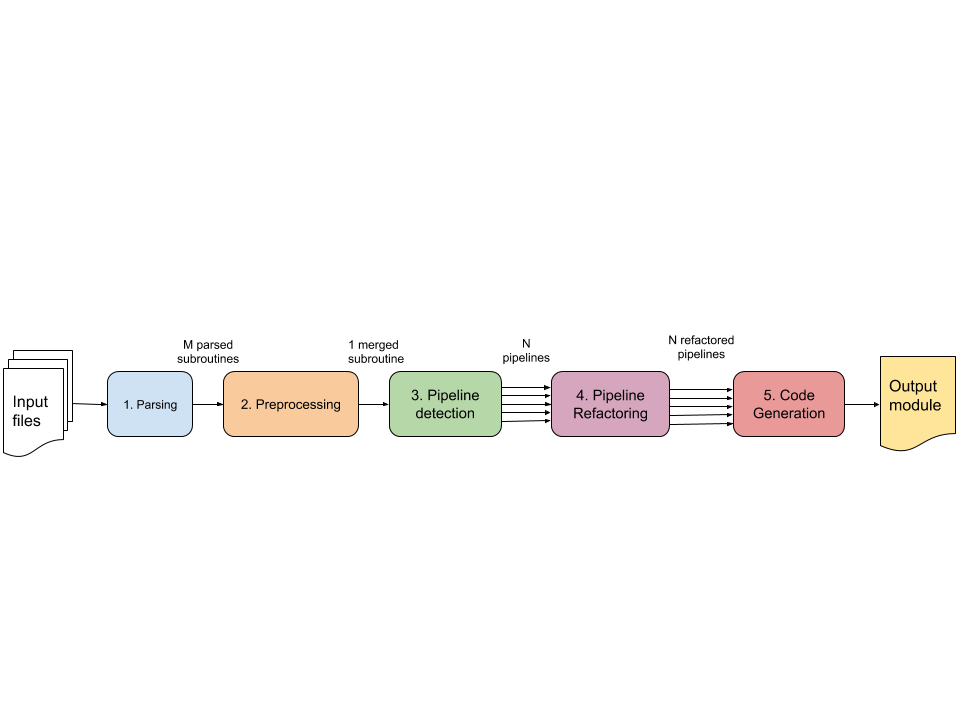
\includegraphics[scale=0.5]{images/Compilation_flow.png}
\end{center}
\caption{\label{fig-eg}An example figure stretching over two columns}
\end{figure*}

\bibliographystyle{abbrv}
\bibliography{main.bib}


\end{document}
